\section{Graph shortest path problem}

\subsection*{Dijkstra's algorithm}
Given a directed graph $G=(N,A)$ with a cost $c_j \in R$ for each arc $(i,j) \in A$, and two nodes $s$ and $t$, determine a minimum cost path from $s$ to $t$. 

Each value $c_j$ represents the cost associated with arc $(i,j) \in A$. 
Here, node $s$ is designated as the source or origin, while node $t$ is specified as the destination or sink.
\begin{definition}
    A path is considered \emph{simple} when it ensures that each node is visited exactly once, without any repetitions.
\end{definition}
\begin{property}
    If $c_j \geq 0$ for all $(i,j) \in A$, there is at least one shortest path which is simple. 
\end{property}
Dijkstra's algorithm takes as input a graph $G = (N, A)$ with non-negative arc costs and a designated starting node $s$. 
The primary purpose of this algorithm is to determine the shortest paths from $s$ to all other nodes within $G$.
The algorithm's core principle involves systematically processing nodes based on their increasing order of the cost of the shortest path from s to each of them. 
For each node $j$ belonging to $N$, we assign two labels:
\begin{itemize}
    \item $L_j$, which represents the cost of the minimum-cost path from s to j.
    \item $pred_j$, which identifies the predecessor of $j$ along the shortest path from $s$ to $j$.
\end{itemize} 
It is important to note that Dijkstra's algorithm follows a greedy approach with respect to path from $s$ to $j$. 
\begin{example}
    Let's apply Dijkstra's algorithm to a given graph, starting with node 1 as the initial node. 
    We assign labels as follows:
    \begin{figure}[H]
        \centering
        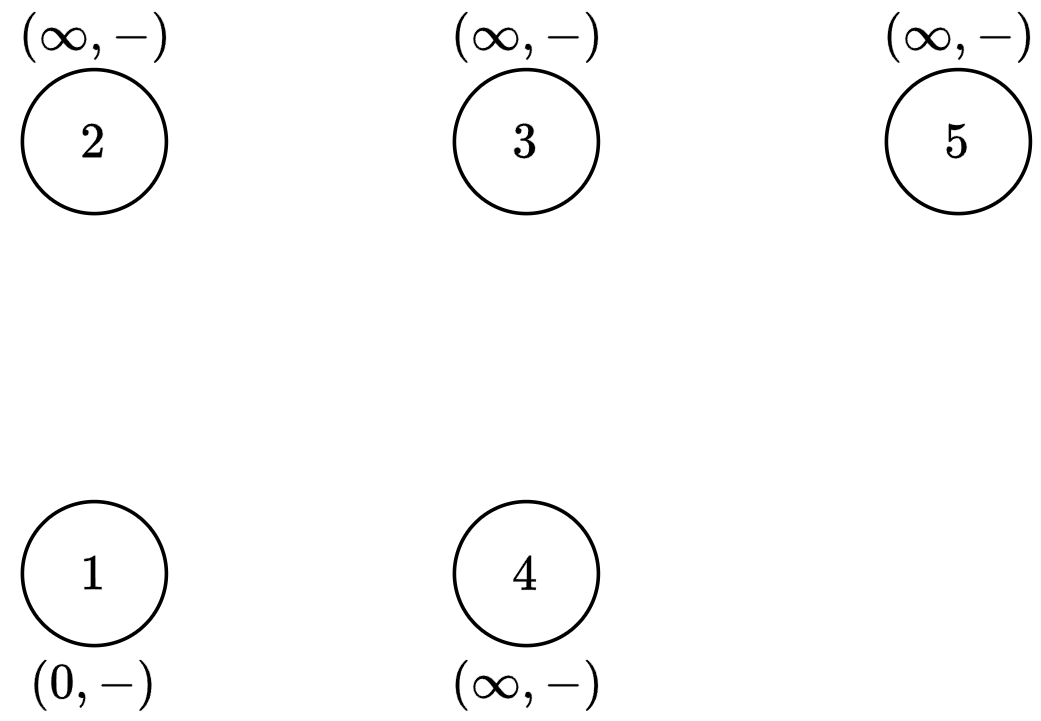
\includegraphics[width=0.2\linewidth]{images/D1.png}
    \end{figure}
    Next, we examine all arcs leading from the starting node to other nodes and update their labels:
    \begin{figure}[H]
        \centering
        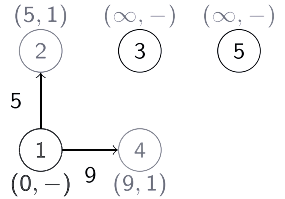
\includegraphics[width=0.2\linewidth]{images/D2.png}
    \end{figure}
    Moving to node 2, we explore reachable nodes. 
    In this case, we find the shortest path from the initial node to 4, so we update the label for 4:
    \begin{figure}[H]
        \centering
        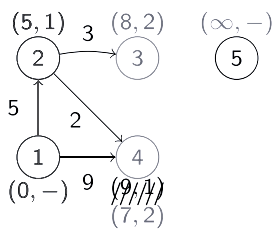
\includegraphics[width=0.2\linewidth]{images/D3.png}
    \end{figure}
    Now, we proceed to node 4, which is the closest node to the starting point.
        We check all arcs leading to other nodes:
    \begin{figure}[H]
        \centering
        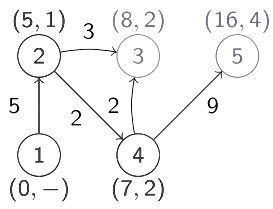
\includegraphics[width=0.2\linewidth]{images/D4.png}
    \end{figure}
    We repeat this process for the remaining nodes, considering them in ascending order of cost from the start:
    \begin{figure}[H]
        \centering
        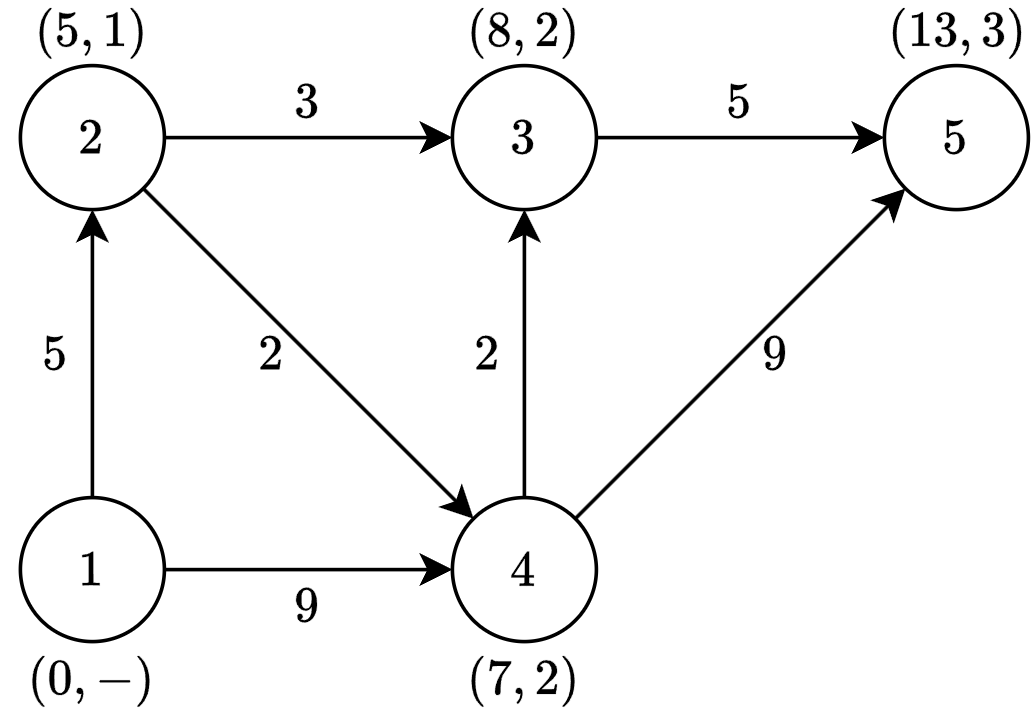
\includegraphics[width=0.4\linewidth]{images/D5.png}
    \end{figure}
    At this point, we can trace back the shortest path to any node in the graph using the predecessor label. 
    For instance, the shortest path from $s$ to 5 has a cost of 13, and the path is $(1,2,3,5)$. 
\end{example}

The inputs to the algorithm consist of a graph $G=(N, E)$ with non-negative costs assigned to its arcs, and a designated starting node $s$, which is a member of $N$.
\begin{algorithm}[H]
    \caption{Dijkstra's algorithm for the graph shortest path problem}
        \begin{algorithmic}[1]
            \State $S \leftarrow \varnothing$
            \State $X \leftarrow \{s\}$
            \For {$u \in N$}
                \State $L_u \leftarrow +\infty$
            \EndFor
            \State $L_s \leftarrow 0$
            \While {$\left\lvert S \right\rvert \neq n$}
                \State $u \leftarrow \textnormal{argmin}\{L_i|i \in X\}$
                \State $X \leftarrow X-\{u\}$
                \State $S \leftarrow S \cup \{u\}$
                \For {$(u,v) \in \delta^{+}(u) \: \textnormal{such that} \: L_v> L_u + c_{uv} $}
                    \State $L_v \leftarrow L_u+c_{uv}$
                    \State $pred_v \leftarrow u$
                    \State $X \leftarrow X \cup \{v\}$
                \EndFor
            \EndWhile
        \end{algorithmic}
\end{algorithm}
The worst-case time complexity of this algorithm is $O(n^3)$. 
\begin{proposition}
    Dijkstra's algorithm is exact. 
\end{proposition}
\begin{proof}
    At the $k$-th step: $S = \{s,i_2,\dots,i_k\}$ and 
    \[L_j=
    \begin{cases}
        \textnormal{cost of a minimum path from } s \textnormal{ to } j,\:j \in S \\ 
        \textnormal{cost of a minimum path with all intermediate nodes in } S, \: j \notin S
    \end{cases}
    \]
    By induction on the number $k$ of steps: 
    \begin{itemize}
        \item Base case: it is easy to see that the statement holds for $k = 1$, since 
            \[S=\{s\},\: L_s=0,\: L_j= +\infty,\: \forall j \neq S \]
        \item Inductive step: we must prove that, if the statement holds at the $k$-th step, it must also hold for the $(k + 1)$-th step. 
    \end{itemize}
    In the $(k + 1)$-th step let $u \notin S$be the node that is inserted in $S$ and $\varnothing$ the path from $s$ to $u$ such that:
    \[L_v + c_{uv} \leq L_i + C_{ij},\: \forall(i,j) \in \delta^{+}(S)\]
    Let us verify that every path $\pi$ from $s$ to $u$ has $c(\pi) \geq c(\varnothing)$. There exist $i \in S$ and $j \notin S$ such that: 
    \[\pi= \pi_1 \cup \{(i,j)\} \cup \pi_2\]
    Where $(i, j)$ is the first arc in $\pi \cap \delta^{+}(S)$. Moreover: 
    \[c(\pi) = c(\pi_1) + c_{ij} + c(\pi_2) \geq L_i + c_{ij}\]
    Because $c_{ij} \geq 0$, thus, $c(\pi_2) \geq 0$, and by the induction assumption, $c(\pi_1) \geq L_i$. Finally, by the choice of $(v,u)$ we have: 
    \[L_i + c_{ij} \geq L_v + c_{vu} = c(\varnothing)\]
\end{proof}
We can observe the following points:
\begin{itemize}
    \item A collection of the shortest paths from the starting node $s$ to all nodes $j$ can be obtained using the predecessor vector.
    \item The union of a set of the shortest paths from node $s$ to all the other nodes of $G$ is the shortest path trees rooted at $s$. 
        These shortest path trees are distinct from minimum-cost spanning trees.
    \item Dijkstra's algorithm is not applicable when there are arcs with negative costs.
\end{itemize}

\subsection*{Floyd-Warshall's algorithm}
When the graph $G$ contains a negative-cost cycle, the well-defined nature of the shortest path problem is compromised. 
Such cycles repeatedly lead to a decrease in cost, making it impossible to identify a finite shortest path from node $s$ to $t$.
To address this issue, the Floyd-Warshall algorithm is employed, as it is capable of detecting negative-cost cycles.
The Floyd-Warshall algorithm provides a comprehensive set of shortest paths between all pairs of nodes, even in the presence of arcs with negative costs. 
This algorithm is founded on an iterative process known as a triangular operation.
It employs $n \times n$ matrices, $D$ and $P$, where their elements represent, upon completion of the algorithm:
\begin{itemize}
    \item $d_{ij}$, denoting the cost of the shortest path from node $i$ to $j$.
    \item $p_{ij}$, indicating the predecessor of node $j$ in the shortest path from node $i$ to $j$.
\end{itemize}

\begin{definition}
    The \emph{triangular operation} specifies that for every pair of nodes $i$ and $j$, where $i$ is not equal to $u$ and $j$ is not equal to $u$ (including the case when $i$ equals $j$), one should examine whether it is more advantageous to reach $j$ from $i$ via an intermediate node $u$. 
    This determination is made by checking if the following relationship holds:
    \[d_{iu}+d_{uj} < d_{ij}\]
\end{definition}

\begin{example}
    Consider the following graph:
    \begin{figure}[H]
        \centering
        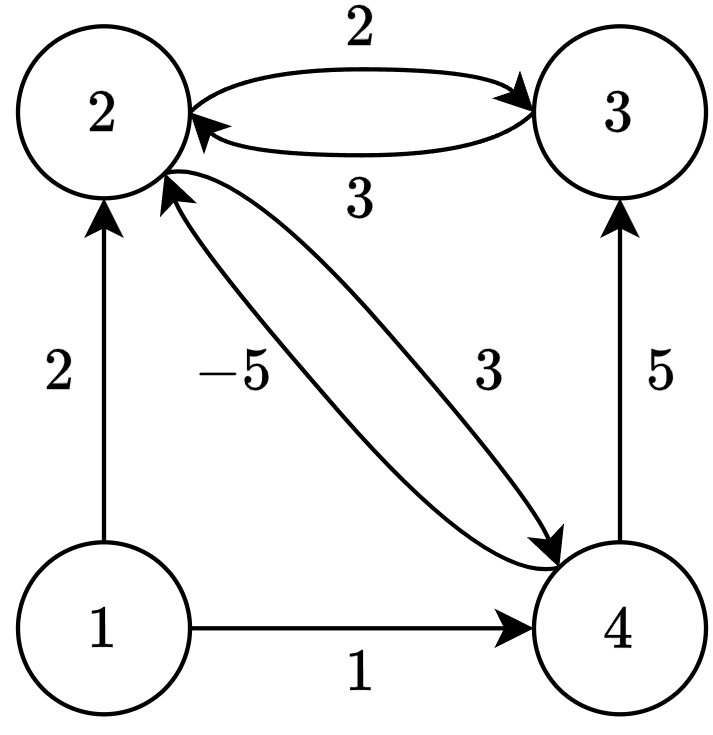
\includegraphics[width=0.2\linewidth]{images/floyd.png}
    \end{figure}
    To initiate the algorithm, we initialize the matrices as follows:
    \[D=\begin{bmatrix}
        0 & 2 & \infty & 1 \\
        \infty & 0 & 3 & 3 \\
        \infty & 2 & 0 & \infty \\
        \infty & -5 & 5 & 0 \\
    \end{bmatrix}
    \:\:\:\:\:\:
    P=\begin{bmatrix}
        1 & 1 & 1 & 1 \\
        2 & 2 & 2 & 2 \\
        3 & 3 & 3 & 3 \\
        4 & 4 & 4 & 4 \\
    \end{bmatrix}
    \]
    In the first iteration with $u=1$ (we focus on the first row and first column), the matrices remain unchanged because the triangular operation is consistently satisfied:
    \begin{itemize}
        \item $0=d_{22} < d_{21} + d_{12} = \infty + 2$ (no changes). 
        \item $3=d_{23} < d_{21} + d_{13} = \infty + \infty$ (no changes). 
        \item $3=d_{24} < d_{21} + d_{14} = \infty + 1$ (no changes). 
        \item $2=d_{32} < d_{31} + d_{12} = \infty + 2$ (no changes). 
        \item $0=d_{33} < d_{31} + d_{13} = \infty + \infty$ (no changes). 
        \item $\infty=d_{34} < d_{31} + d_{14} = \infty + 1$ (no changes). 
        \item $-5=d_{42} < d_{41} + d_{12} = \infty + 2$ (no changes). 
        \item $5=d_{43} < d_{41} + d_{13} = \infty + \infty$ (no changes). 
        \item $0=d_{44} < d_{41} + d_{14} = \infty + 1$ (no changes). 
    \end{itemize}
    In the second iteration with $u=2$ (focusing on the second row and second column), the matrices are modified, and the algorithm terminates due to the discovery of a negative-cost arc:
    \begin{itemize}
        \item $0=d_{11} < d_{12} + d_{21} = 2 +\infty $ (no changes). 
        \item $\infty=d_{13} < d_{12} + d_{23} = 2+3$ ($p_{13} \leftarrow p_{23}$). 
        \item $1=d_{14} < d_{12} + d_{24} = 2+3$ (no changes). 
        \item $\infty=d_{31} < d_{32} + d_{21} = 2 + \infty$ (no changes). 
        \item $0=d_{33} < d_{32} + d_{23} = 2+3$ (no changes). 
        \item $\infty=d_{34} < d_{32} + d_{24} = 2+3$ ($p_{34} \leftarrow p_{24}$). 
        \item $\infty=d_{41} < d_{42} + d_{21} = 5 + \infty$ (no changes). 
        \item $5=d_{43} < d_{42} + d_{23} = -5+3$ ($p_{43} \leftarrow p_{23}$). 
        \item $0=d_{44} < d_{42} + d_{24} = -5+3$ (negative cost circuit found). 
    \end{itemize}
\end{example}

The algorithm takes as its inputs a directed graph $G = (N,A)$ and an $n \times n$ cost matrix, $C = [c_{ij}]$.
\begin{algorithm}[H]
    \caption{Floyd-Warshall's algorithm}
        \begin{algorithmic}[1]
            \For {$i \in N$}
                \For {$j \in N$}
                    \State $p_{ij} \leftarrow i$
                    \State $d_{ij} \leftarrow \begin{cases}
                        0 \:\:\:\:\:\:\:\:\:\:\: i = j \\
                        c_{ij} \:\:\:\:\:\:\:\:\: i \neq j \land (i,j) \in A \\
                        +\infty \:\:\:\:\:\: \textnormal{otherwise}
                    \end{cases}$
                \EndFor
            \EndFor
            \For {$u \in N$}
                \For {$i \in N-\{u\}$}
                    \For {$j \in N-\{u\}$}
                        \If {$d_{iu}+d_{uj} \ d_{ij}$}
                            \State $p_{ij} \leftarrow p_{uj}$
                            \State $d_{ij} \leftarrow d_{iu}+d_{uj}$
                        \EndIf
                    \EndFor
                \EndFor
                \For {$i \in N$}
                    \If {$d_{ii} < 0$}
                        \State \Return
                    \EndIf
                \EndFor
            \EndFor
        \end{algorithmic}
\end{algorithm}
Given that the triangular operation is executed for all nodes $u$ and for each pair of nodes $i$ and $j$ in the worst-case scenario, the overall time complexity of the Floyd-Warshall algorithm is $O(n^3)$.
\begin{proposition}
    Floyd-Warshall's algorithm is exact. 
\end{proposition}
\begin{proof}
    Let's assume that the nodes of $G$ are numbered from $1$ to $n$. 
    We can verify that when following the node index order, after the $u$-th cycle, the value of $d_{ij}$ (for any $i$ and $j$) corresponds to the cost of the shortest path from $i$ to $j$ with only intermediate nodes in the set ${1,\dots,u}$. 
\end{proof}

\subsection*{Topological order algorithm}
The topological order algorithm deals with a directed acyclic graph $G = (N,A)$, where each arc $(i,j) \in A$ has an associated cost $c_ij \in \mathbb{R}$, 
Given nodes $s$ and $t$, the goal is to determine the shortest or longest path from $s$ to $t$.
Directed acyclic graphs possess a crucial property known as topological order, where the nodes in any such graph $G$ can be indexed in a way that for each arc $(i, j) \in A$, we have $i < j$. 
This topological order property can be leveraged in an efficient dynamic programming algorithm to find shortest or longest paths in directed acyclic graphs.
To apply the algorithm to a graph $G = (N,A)$, represented using lists of predecessors $\delta^{-}(v)$ and successors $\delta^{+}(v)$ for each node $v$, follow these steps:
\begin{enumerate}
    \item Assign the smallest positive integer that has not been assigned to a node $v \in N$ with $\delta^{-}(v)=\varnothing$. 
    \item Delete node $v$ with all its incident arcs.
    \item Repeat from step one until there are nodes remaining in the current sub-graph.
\end{enumerate}
The complexity of this algorithm is $O(m)$, where $m$ is the cardinality of $A$ (the number of arcs), because each node and arc are considered at most once.
\begin{example}
    Here's a graphical illustration of the algorithm:
    \begin{figure}[H]
        \centering
        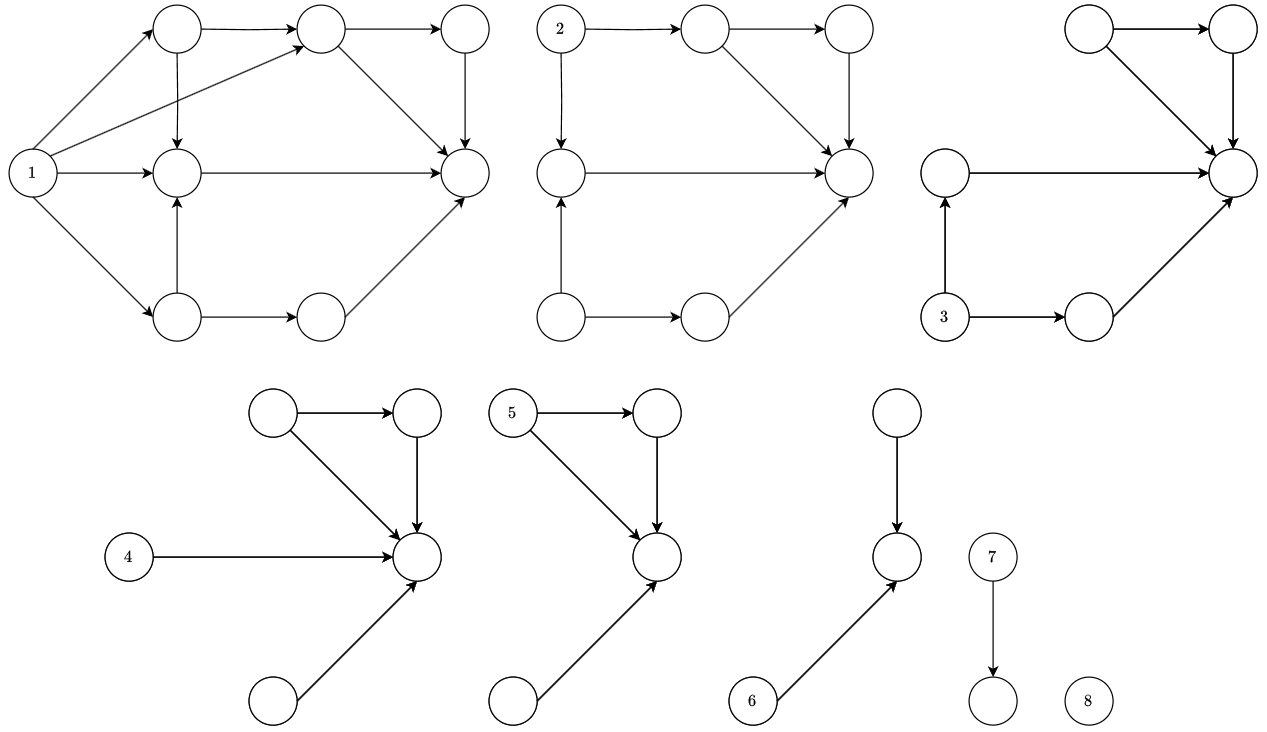
\includegraphics[width=0.8\linewidth]{images/spath.png}
    \end{figure}
\end{example}

\subsection*{DAGs' dynamic programming algorithm}
Any shortest path from 1 to $\pi_t$, with at least two arcs, can be subdivided into two parts: $\pi_t$ and $(i,t)$, where $\pi_t$ is the shortest sub-path from $s$ to $i$. 
For each node  $i=1,\dots,t$, let $L_i$ denote the cost of the shortest path from $1$ to $i$. 
Therefore, we can express $L_t$as follows:
\[L_t=\min_{(i,t) \in \delta^{-}(t)}\{L_i+c_{it}\}\]
This minimum is taken over all possible predecessors $i$ of $t$.
If the graph $G$ is directed, acyclic, and topologically ordered, the only possible predecessors of $t$ in the shortest path $\pi_t$ from 1 to $t$ are those nodes with an index $i$ less than $t$. 
Consequently:
\[L_t=\min_{i<t}\{L_i+c_{it}\}\]
However, in a graph with cycles, any node other than $t$ can be a predecessor of $t$ in $\pi_t$.  

For Directed Acyclic Graphs (DAGs) whose nodes are topologically ordered, $L_{t-1},\dots,_L1$ satisfy the same type of recursive relations:
\[L_{t-1}=\min_{i<t-1}\{L_i+c_{i,t-1}\};\dots;L_2=\min_{i=1}\{L_i+c_i2\}=L_1+c_{12};L_1=0\]
These relations can be solved in reverse order:
\[L_1=0;L_2=L_1+c_{12};\dots;L_{t}=\min_{i<t-1}\{L_i+c_{t}\}\]
\begin{example}
    Consider the following graph:
    \begin{figure}[H]
        \centering
        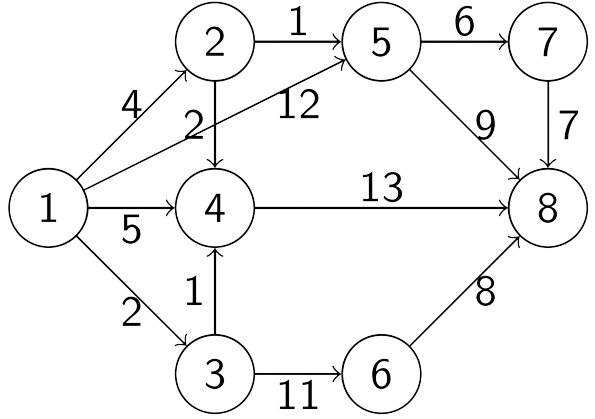
\includegraphics[width=0.4\linewidth]{images/DAG.png}
    \end{figure}
    To find the shortest paths in a Directed Acyclic Graph (DAG) using dynamic programming, follow this workflow:
    \begin{itemize}
        \item $L_1=0 \rightarrow \textnormal{pred}_1=1$
        \item $L_2=L_1+c_{12}=4 \rightarrow \textnormal{pred}_2=1$
        \item $L_3=L_1+c_{13}=2 \rightarrow \textnormal{pred}_3=1$
        \item $L_4=\min_{i=1,2,3}\{L_i+c_{i4}\}=\min{5,6,3}=3 \rightarrow \textnormal{pred}_4=3$
        \item $L_5=\min_{i=1,2}\{L_i+c_{i5}\}=\min{12,5}=5 \rightarrow \textnormal{pred}_5=2$
        \item $L_6=L_3+c_{36}=13 \rightarrow \textnormal{pred}_6=3$
        \item $L_7=L_5+c_{57}=11 \rightarrow \textnormal{pred}_7=5$
        \item $L_8=\min_{i=4,5,6,7}\{L_i+c_{i8}\}=\min{16,14,21,18}=14 \rightarrow \textnormal{pred}_8=5$
    \end{itemize}
\end{example}
\begin{algorithm}[H]
    \caption{Dynamic programming to find the shortest paths in DAGs}
        \begin{algorithmic}[1]
            \State Sort the nodes of $G$ topologically
            \State $L_1 \leftarrow 0$
            \For {$j=2,\dots,n$}
                \State $L_j \leftarrow \min\{L_i+c_{ij}|(i,j) \in \delta^{-}(j) \land i < j\}$
                \State $pred_j \leftarrow v \: \textnormal{such that} \: (v,j)=\textnormal{argmin} \{L_i+c_{ij}|(i,j) \in \delta^{-}(j) \land i < j\}$
            \EndFor
        \end{algorithmic}
\end{algorithm}
As the nodes are topologically ordered, each node and each arc is processed exactly once, resulting in a time complexity of $O(m)$, where $m$ represents the cardinality of $A$ (the number of arcs).    

The same algorithm can also be applied to find the longest path using the following formula:
\[L_t=\max_{i<t}\{L_i+c_{it}\},\dots\]

\begin{proposition}
    The dynamic programming algorithm for DAGs is exact. 
\end{proposition}
\begin{proof}
    This phenomenon can be attributed to the optimality principle.
    For any shortest (longest) path from node from 1 to $t,\pi_t$, there exists a pair of nodes $i$ and $j$, where $i < j$,  such that the path can be partitioned into two parts: $\pi_i$ and $(i,t)$, where $\pi_i$ represents the minimum (maximum) length from $s$ to $i$.
\end{proof}

\subsection*{Project planning algorithm}
\begin{definition}
    A \emph{project}  comprises a collection of $m$ activities with an associated duration. 
    Specifically, activity $A_i$ has an estimated duration of $d_j \geq 0, i=1,\dots,m$. 

    Certain pairs of activities are governed by \emph{precedence constraint}. 
    A notation such as $A_i \varpropto A_j$ signifies that the commencement of $A_j$ is contingent upon the completion of $A_i$. 
\end{definition}
A project can be conveniently represented using a directed graph $G = (N, A)$, where each arc corresponds to an activity, and the length of the arc signifies the duration of the associated activity.
In order to account for the precedence constraints, the arcs must be arranged in a manner such that the notation $A_i \varpropto A_j$ implies the existence of a directed path where the arc associated with $A_i$ precedes the arc associated with $A_j$.
This ensures the proper sequencing of activities.
In this context, a node $v$ marks an event corresponding to the end of all the activities $(i,v) \in \delta^{-}(v)$, consequently, it indicates the potential beginning of all activities $(v,j) \in \delta^{+}(v)$. 
To enhance the representation of graph $G$ we use additional nodes that adheres to the following criteria:
\begin{itemize}
    \item It includes a distinct initial node $s$, symbolizing the project's start event.
    \item It incorporates a unique final node $t$, representing the project's completion event.
    \item It maintains a structure where multiple arcs with the same endpoints are avoided, ensuring clarity and consistency in the representation. 
\end{itemize}
\begin{property}
    The directed graph G representing any project is acyclic (it is a DAG). 
\end{property}
\begin{proof}
    By contradiction, if $A_{i1}\varpropto A_{12},\dots,A_{jk}\varpropto A_{ki}$ there would be a logical inconsistency. 
\end{proof}  
\begin{example}
    A project can be described as follows:
    \begin{figure}[H]
        \centering
        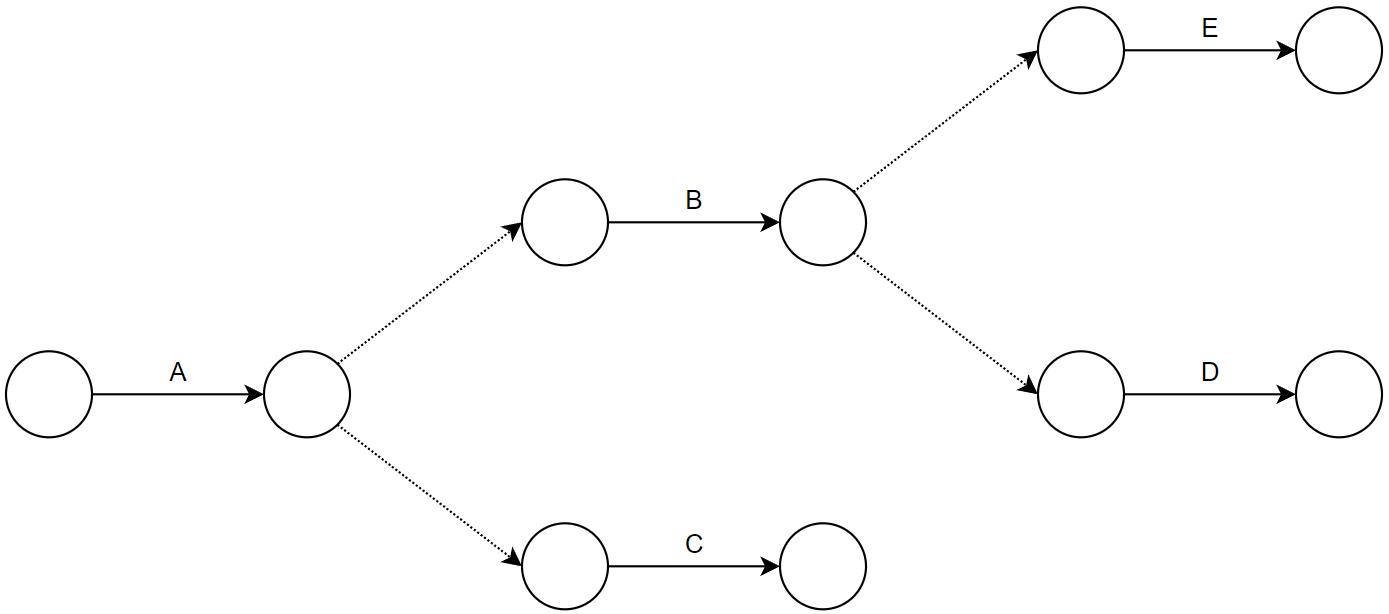
\includegraphics[width=0.5\linewidth]{images/project.png}
    \end{figure}
    While it is possible to simplify this graph by contracting some arcs, care must be taken to avoid introducing unwanted precedence constraints. 
    The correctly contracted graph appears as follows:
    \begin{figure}[H]
        \centering
        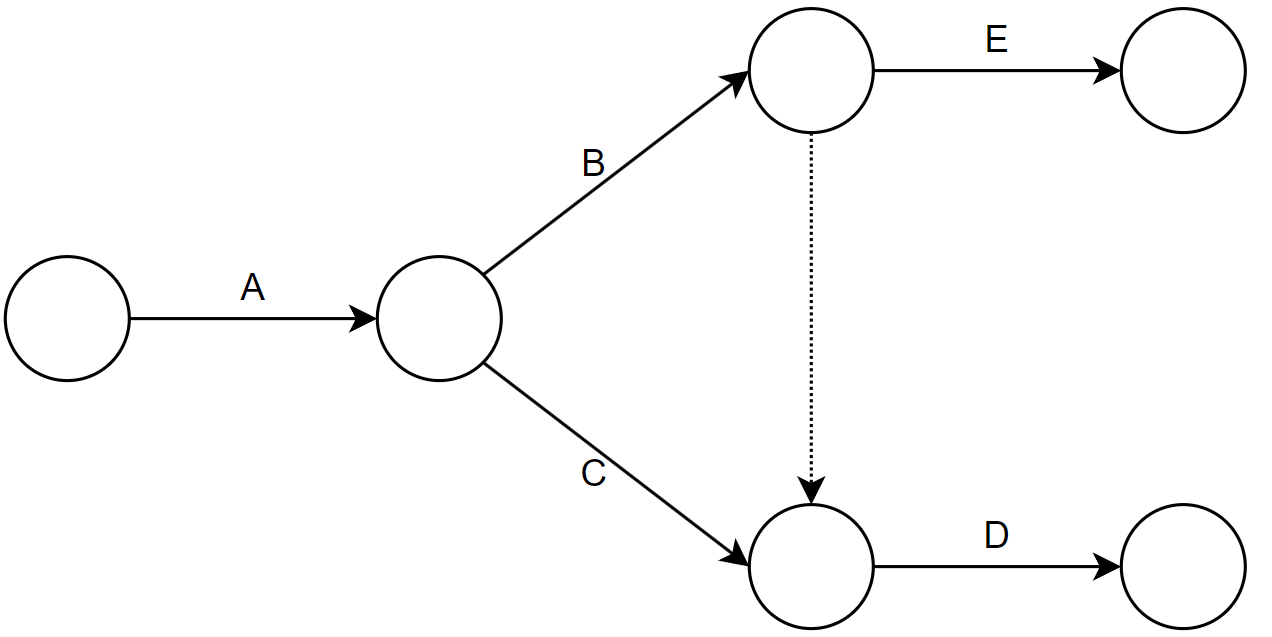
\includegraphics[width=0.4\linewidth]{images/cproject.png}
    \end{figure}
    Additionally, we can introduce the initial and final nodes to create a more structured representation:
    \begin{figure}[H]
        \centering
        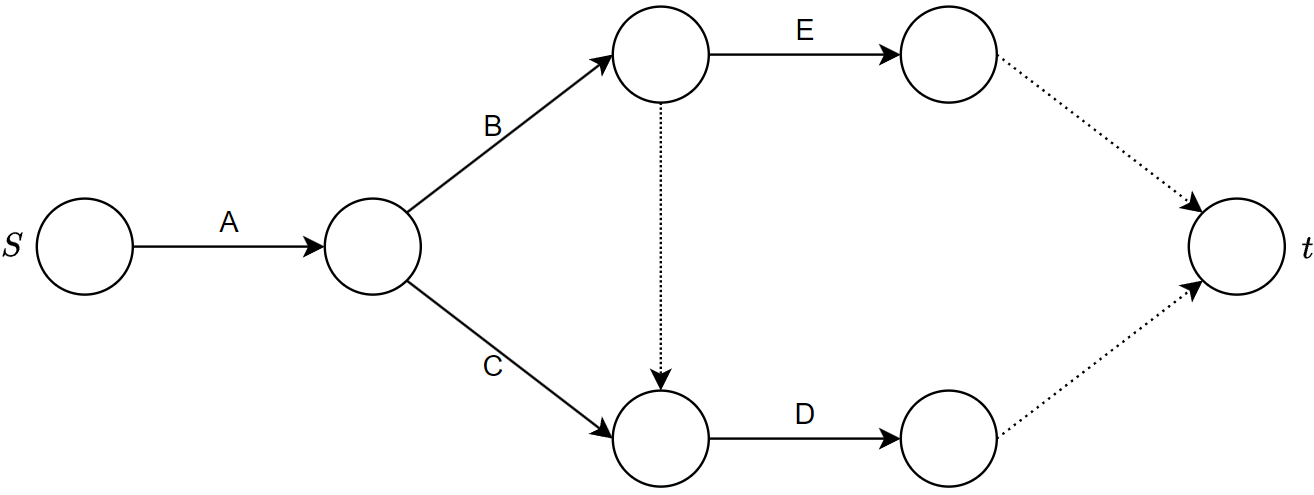
\includegraphics[width=0.5\linewidth]{images/fproject.png}
    \end{figure}
\end{example}
The problem to be addressed is as follows: given a project, the task is to schedule the activities in a manner that minimizes the total duration of the project.
\begin{property}
    The minimum overall project duration is the length of the longest path from $s$ to $t$. 
\end{property}
\begin{proof}
    Since any $s-t$ path represents a sequence of activities that must be executed in the specified order, its length provides a lower bound on the minimum overall project duration. 
\end{proof}  
To address this problem, we can employ the Critical Path Method (CPM), which accomplishes the following:
\begin{itemize}
    \item Establishes a schedule to minimize the overall project duration.
    \item Determines the slack for each activity.
\end{itemize}
The algorithm takes as input the project's representation graph $G$ and seeks to identify a topological order of the nodes. 
The steps involved are as follows:
\begin{enumerate}
    \item Traverse the nodes in ascending order of indices.
        For each node $h \in N$, calculate the earliest time, denoted as $T_{min_h}$, at which the event associated with node $h$ can occur ($T_{min_n}$ corresponds to the minimum project duration).
    \item Traverse the nodes in descending order of indices.
        For each node $h \in N$, compute the latest time, denoted as $T_{max_h}$, at which the event associated with node h can occur without causing a delay in the project's completion beyond $T_{min_n}$.
    \item For each activity $(i,j) \in A$, determine the slack, denoted as $\sigma_{ij}$, using the formula: 
        \[\sigma_{ij}=T_{max_j}-T_{max_i}-d_{ij}\]
\end{enumerate}
\begin{example}
    Consider the following project:
    \begin{table}[H]
        \centering
        \begin{tabular}{ccc}
        \hline
        \textbf{Activity} & \textbf{Duration} & \textbf{Predecessors} \\ \hline
        A                 & 3                 & -                     \\
        B                 & 2                 & A                     \\
        C                 & 3                 & A                     \\
        D                 & 3                 & C                     \\
        E                 & 4                 & B, C                  \\
        F                 & 3                 & B                     \\
        G                 & 1                 & E, D                  \\
        H                 & 4                 & C                     \\
        I                 & 2                 & F                     \\ \hline
        \end{tabular}
    \end{table}
    With the following precedence constraints:
    \[A \varpropto B,A \varpropto C,C \varpropto D,B \varpropto E, C \varpropto E,B \varpropto F,E \varpropto G,D \varpropto G,C \varpropto H,F \varpropto I\]
    The objective is to determine the minimum overall duration of the project and calculate the slack for each activity. 
    To do this, we start by creating a graph associated with the given problem:
    \begin{figure}[H]
        \centering
        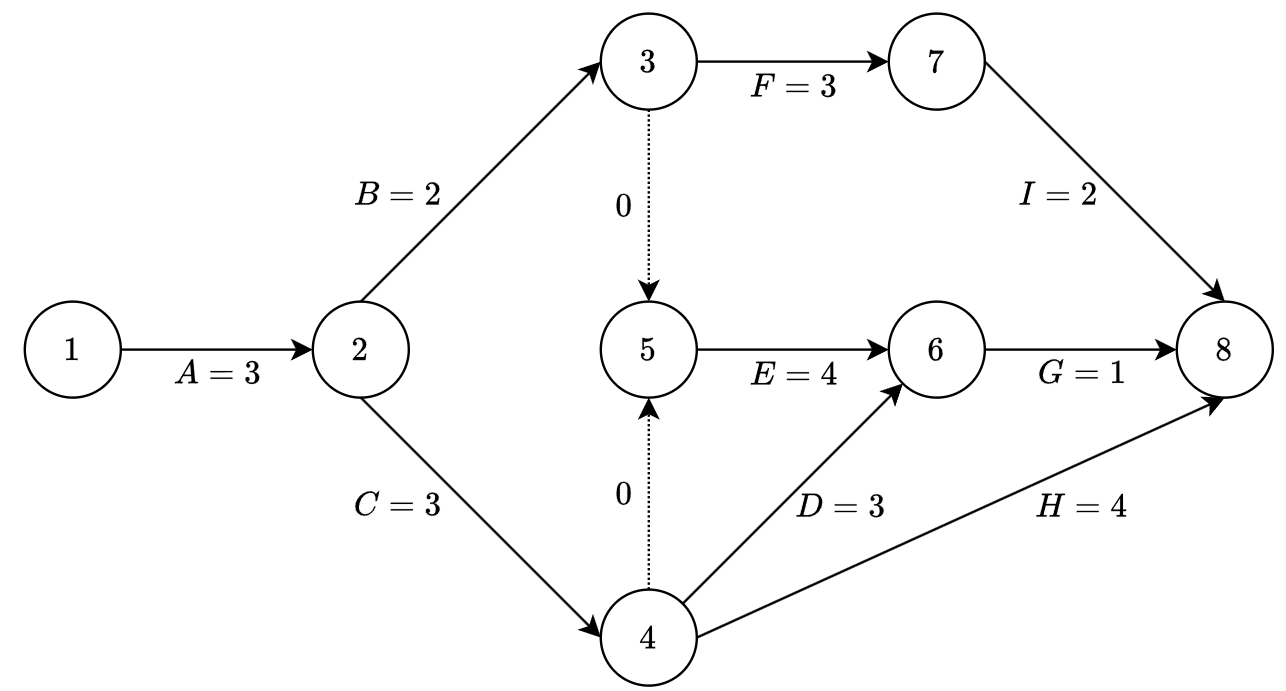
\includegraphics[width=0.5\linewidth]{images/eproject.png}
    \end{figure}
    The first two phases of the CPM algorithm result in the following graphs:
    \begin{figure}[H]
        \centering
        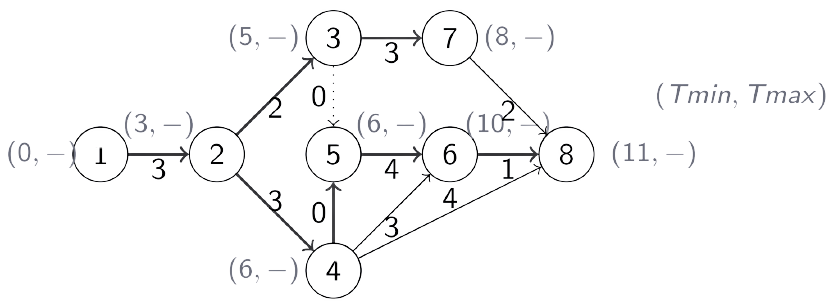
\includegraphics[width=0.75\linewidth]{images/aproject.png}
    \end{figure}
    \begin{figure}[H]
        \centering
        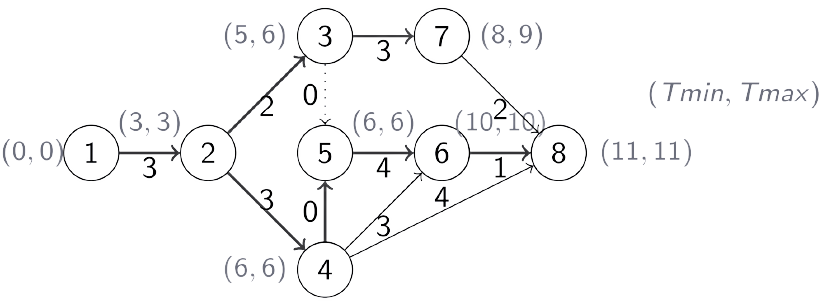
\includegraphics[width=0.75\linewidth]{images/aproject1.png}
    \end{figure}
    As a result, the longest path that is critical, and hence determines the minimum project duration, is $(1,2,4,5,6,8)$.
\end{example}
The algorithm takes as inputs a graph $G = (N,A)$, where $n= \left\lvert N \right\rvert $, and the duration $d_{ij}$ assigned to each $(i,j) \in A$. 
\begin{algorithm}[H]
    \caption{Algorithm for the critical path method}
        \begin{algorithmic}[1]
            \State Sort the nodes of $G$ topologically
            \State $T_{min_1} \leftarrow 0$
            \For {$j=2,\dots,n$}
                \State $T_{min_j} \leftarrow \max\{T_{min_i}+d_{ij}|(i,j) \in \delta^{-}(j)\}$
            \EndFor
            \State $T_{max_n} \leftarrow T_{min_n}$
            \For {$i=n-1,\dots,1$}
            \State $T_{max_j} \leftarrow \min\{T_{max_j}-d_{ij}|(i,j) \in \delta^{+}(j)\}$
            \EndFor
        \end{algorithmic}
\end{algorithm}
The algorithm's time complexity is $O(m)$, where $m =\left\lvert A\right\rvert$. 
\begin{definition}
    An activity $(i,j)$ with zero slack, which means that:
    \[\sigma_{ij}=T_{max_j}-T_{min_i}-d_{ij}=0\]
    is considered \emph{critical}. 

    A \emph{critical path} is defined an $s-t$ path only composed of critical activities (it always exists).
\end{definition}

To determine the slack of a project, another approach is to use Gantt charts, which were initially introduced by Henry Gantt in 1910. 
These charts offer a visual representation of the project's timeline.
\begin{example}
    The outcome of the previous example is as follows:
    \begin{table}[H]
        \centering
        \begin{tabular}{cccc}
        \hline
        $(i,j)$ & $d_{ij}$ & $T_{min_i}$ & $T_{max_j}$ \\ \hline
        A       & 3        & 0           & 3           \\
        B       & 2        & 3           & 6           \\
        C       & 3        & 3           & 6           \\
        D       & 3        & 6           & 10          \\
        E       & 4        & 6           & 10          \\
        F       & 3        & 5           & 9           \\
        G       & 1        & 10          & 11          \\
        H       & 4        & 6           & 11          \\
        I       & 2        & 8           & 11          \\ \hline
        \end{tabular}
    \end{table}
    These results can be illustrated using a Gantt chart as shown below:
    \begin{figure}[H]
        \centering
        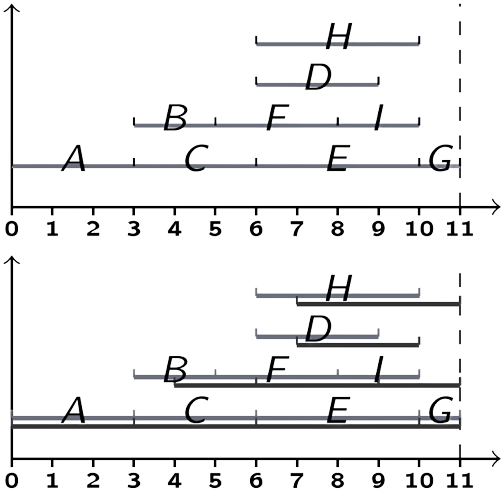
\includegraphics[width=0.25\linewidth]{images/Gantt.png}
    \end{figure}
\end{example}